\documentclass{article}

\usepackage[top=3cm, bottom=3cm, left=3cm, right=3cm]{geometry}

\usepackage[french]{babel}
\usepackage[utf8]{inputenc}
\usepackage[T1]{fontenc}

\usepackage[a4paper,colorlinks,linkcolor=darkgray,citecolor=red,urlcolor=blue]{hyperref}
\usepackage{pdfpages}
\usepackage{graphicx}
\usepackage{caption}
\usepackage{tikz}
\usetikzlibrary{positioning,shapes,arrows,automata}
\tikzset{>=stealth'}
\usepackage{amsthm}

\newtheorem{ex}{Exemple}

\title{Rapport d'activité mi-parcours : TriComp}

\author{}

\date{4 Novembre 2014}

\begin{document}

\makeatletter % Pour utiliser le "at" comme une commande interne.
  \begin{titlepage}
    \begin{center}
       {\LARGE \@title} \\
       \vspace{2cm}
       {\large \@date}
       \vspace{3cm}
    \end{center}
       {\large
       {William \textsc{Aufort} \hfill Julien \textsc{Bensmail} \\}
    \vspace{1cm}
       {\hfill coordinateur \\}
       {Agathe \textsc{Herrou}  \hfill Romain \textsc{Labolle} \\}
       \vspace{1cm}
       {chef de projet \\}
       \vspace{1.5cm}
       {Frédéric \textsc{Lang} \hfill Maxime \textsc{Lesourd} \\}
       {Laureline \textsc{Pinault} \hfill Léo \textsc{Stéfanesco} \\}}
       \vspace{2.5cm}
    \begin{abstract}
	Ce document présente le rapport d'activité mi-parcours de notre projet TriComp. Y sont détaillés le travail fourni jusqu'à présent
dans les différents groupes de travail ainsi que les diverses modifications qui ont été effectuées par rapport à la proposition de projet.
    \end{abstract}
  \end{titlepage}
\makeatother


\newpage

\tableofcontents

\newpage

% Plan (proposition) :
%  I] Travail fourni
%     a) Définition des différents langages
%     b) Interface graphique et site web
%     c) Divers(organisation,...)
%  II] Changements par rapport à la proposition
%     a) Calendrier
%     b) Précisions diverses

\section{Travail fourni}

Nous exposons dans cette partie le travail fourni jusqu'à présent dans les différents groupes de travail.

\subsection{Définition des différents langages}

L'étape cruciale de définition des langages a été effectuée. Nous exposons ici avec précision ces différents langages.

\subsubsection{Instructions utilisateurs}

Une première version du langage des instructions utilisateurs a été établie, avec des tests sur des exemples. Nous avons maintenant des outils
suffisants pour expliquer comment tricoter un modèle simple, dans notre cas rectangulaire avec un motif régulier (comme par exemple une écharpe).

Concrètement, une description bas-niveau d'un tricot, quasiment identique aux instructions utilisateurs, mais en langage machine, existe : le tricot
est ici vu comme un type OCaml. Depuis cette description, un traducteur permet de transformer cela en instructions en français pour réaliser le tricot.

\begin{ex}
  Suivez les instructions suivantes pour obtenir votre tricot : 
  
  \begin{itemize}
  \item Rang 1 : Tricotez un point vide, et répétez 12 fois ce motif. 
  \item Rang 2 : Tricotez un point endroit puis un point envers, et répétez 12 fois ce motif. 
  \item Rang 3 : Tricotez un point envers puis un point endroit puis un point envers, et répétez 8 fois ce motif. 
  \item Rang 4 : Tricotez un point envers puis un point endroit, et répétez 2 fois ce motif. 
  \item Tricotez un point endroit puis un point envers, et répétez 2 fois ce motif. 
  \item Tricotez au total 10 fois ces 4 rangs.
  \end{itemize}
\end{ex}

\subsubsection{Langage descriptif}

Le langage descriptif permet d'interfacer le traducteur et l'interface graphique. Les contraintes étaient d'avoir un format de description facilement manipulable à travers l'interface graphique tout en gardant la structure d'un tricot. La solution adoptée est de voir un tricot comme un assemblage d'éléments qui sont des structures arborescentes de trapèzes tricotés. Ces trapèzes sont tricotés selon divers motifs, pour le moment en point endroit ou envers.

% Si quelqu'un est capable de faire une figure avec le poncho qui avait été dessiné au tableau on peut mettre un exemple de fichier .tricot?

Une syntaxe a été définie et le parser utilisé par le traducteur a été implémenté.


\subsection{Interface graphique}

Nous détaillons dans cette section les fonctionnalités implémentées jusqu'à présent au niveau de l'interface graphique.

\subsubsection{Squelette de l'interface / Aspect}

La première étape du développement de l'interface a été la mise en place de son squelette. Plus précisement, nous avons défini l'aspect
général de l'interface ainsi que les différents outils que nous souhaitons mettre à disposition. Ces outils sont représentés à l'aide de
boutons ou d'options encore inactives pour la plupart. On distingue notamment :
\begin{itemize}
  \item Les options relatives au logiciel TriComp (choisir un point, faire une tresse...) Ceux-ci peuvent être selectionnés grâce à des
boutons dont l'aspect n'est pas encore fixé, car leur implémentation se fera au fur et à mesure et en fonction de l'avancement global du
projet.
  \item Les options que l'on trouve dans tout logiciel (ouvrir, sauvegarder, quitter, ...). Ces options sont fonctionnelles (ou bientôt
fonctionnelles) car les formats de données pour la sauvegarde ont été définis. Nous travaillons directement sur le format de fichier
associé au langage descriptif. Ce type de fichier portera l'extension \texttt{.tricot}.
\end{itemize}
Ci-dessous on peut observer l'aspect général de la fenêtre principale du logiciel.
% TODO Capture d'ecran pour la fenetre du logiciel. Decommenter la suite.
% \begin{figure}[!h]
%   \begin{center}
%     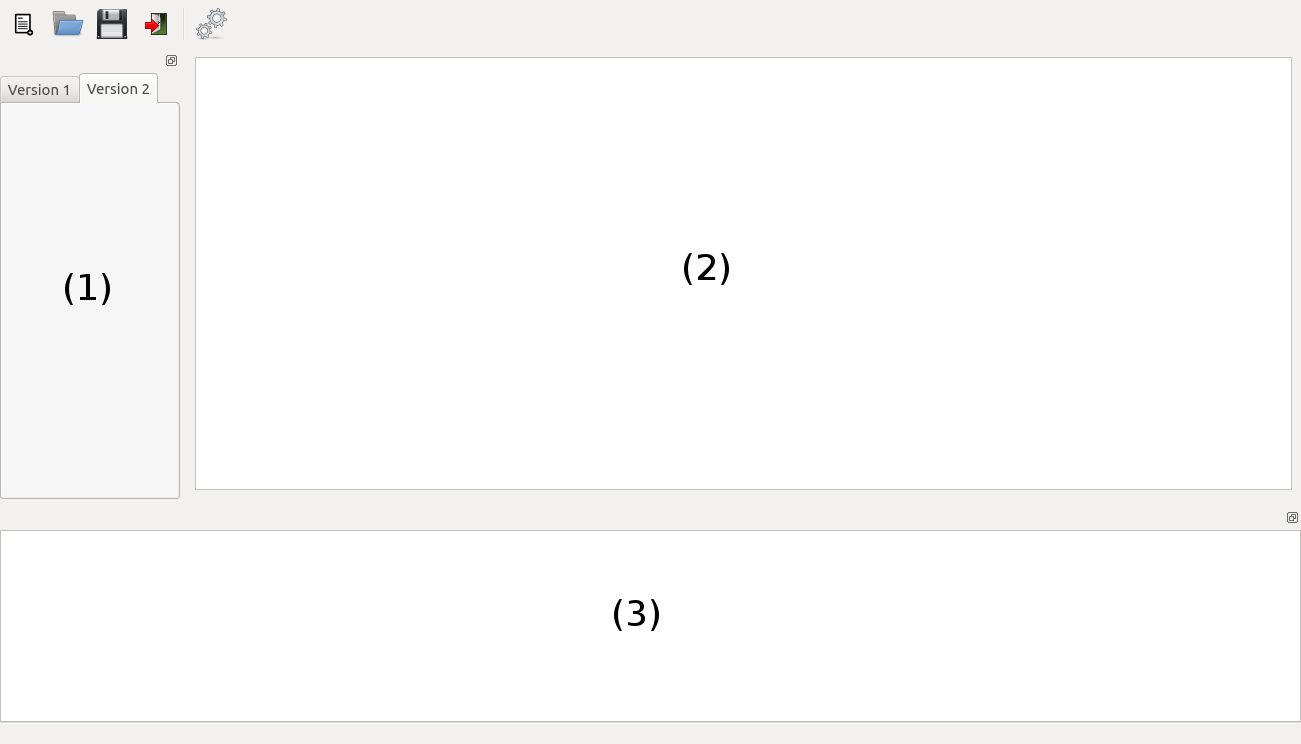
\includegraphics[scale=1]{fenetre.png}
%   \end{center}
% \end{figure}

\subsubsection{Affichage des tricots}

L'affichage des tricots en lui-même est en cours d'implémentation. Il est prévu de les afficher sous forme de patron, avec éventuellement
la possibilité d'afficher la progression d'un tricot en cours de réalisation.
Nous travaillons avec des classes de Qt qui permettent la gestion et l'affichage d'objets 2D (\texttt{QtGraphicsScene} et \texttt
{QtGraphicsItem} par exemple).

\subsection{Site Web}

Un site web a été déployé à l'adresse \url{http://tricomp.github.io}, il est hébergé sur Github (utilisé comme serveur git du projet). Le
site est basé sur Jekyll, un CMS en Ruby spécialisé dans les blogs et qui a la particularité de ne pas utiliser de base de données, avec
l'avantage que Github gère Jekyll automatiquement. Le site est notament une vitrine pour le projet : il en contient une présentation
rapide, avec des liens vers le code source sur Github. A terme, le site sera aussi un support pour télécharger et installer le logiciel
TriComp.

De plus, le site contient pour l'instant un article sur ce qui existe déjà sur Internet autour du tricot (notamment certains projets
proches de TriComp qui ont été détaillés dans la proposition). D'autres articles devrait s'y rajouter, ainsi qu'une page pour aiguiller
rapidement l'internaute anglophone.

\section{Changement par rapport à la proposition}

\subsection{Objectifs}

\subsubsection{Représentation intermédiaire}

Il avait initialement été prévu de développer une représentation intermédiaire, où le tissu serait représenté sous la forme d'un graphe,
dans lequel les sommets correspondraient aux mailles et les arêtes à la manière dont les mailles interagissent. Cette représentation avait
pour but primaire d'aider à la détection de configurations impossibles. Cependant, après avoir approfondi les langages de bas et haut
niveaux, nous nous sommes rendus compte que ce formalisme n'était pas intrinsèquement nécessaire. % Plus d'explications ?
Nous avons donc abandonné l'utilisation globale de cette formalisation, pour ne se concentrer que sur l'étude de motifs impossibles
ponctuelle et non systématique.

\subsection{Calendrier}

\subsection{Précisions diverses}

\section*{Conclusion}

\end{document}
